% ===========================================================================
% Section 5: Results and Analysis
% ===========================================================================

This section presents the main experimental results.
All experiments use $n = 200$ samples per dataset (FinanceBench: $n = 150$, full dataset) unless otherwise noted.
We address three research questions: RQ1 compares \ours{} against baselines (\S\ref{subsec:rq1}), RQ2 analyzes the agent's tool usage patterns (\S\ref{subsec:rq2}), and RQ5 evaluates DSPy optimization effects (\S\ref{subsec:rq5}).
Ablation studies for RQ3 (evaluation tool variants) and RQ4 (structure-aware tools) are presented in \S\ref{sec:ablation}.

% ---------------------------------------------------------------------------
\subsection{RQ1: Agentic vs.\ Baseline Pipelines}
\label{subsec:rq1}
% ---------------------------------------------------------------------------

\textbf{Does ReAct-based agentic refinement improve answer quality compared to fixed-loop refinement and single-pass baselines?}

Table~\ref{tab:rq1_main} and Figure~\ref{fig:rq1_f1} present the main results across four datasets using Gemini Flash Lite.

% Figure: RQ1 F1 Comparison (Gemini Flash Lite, n=200)
\begin{figure*}[t]
\centering
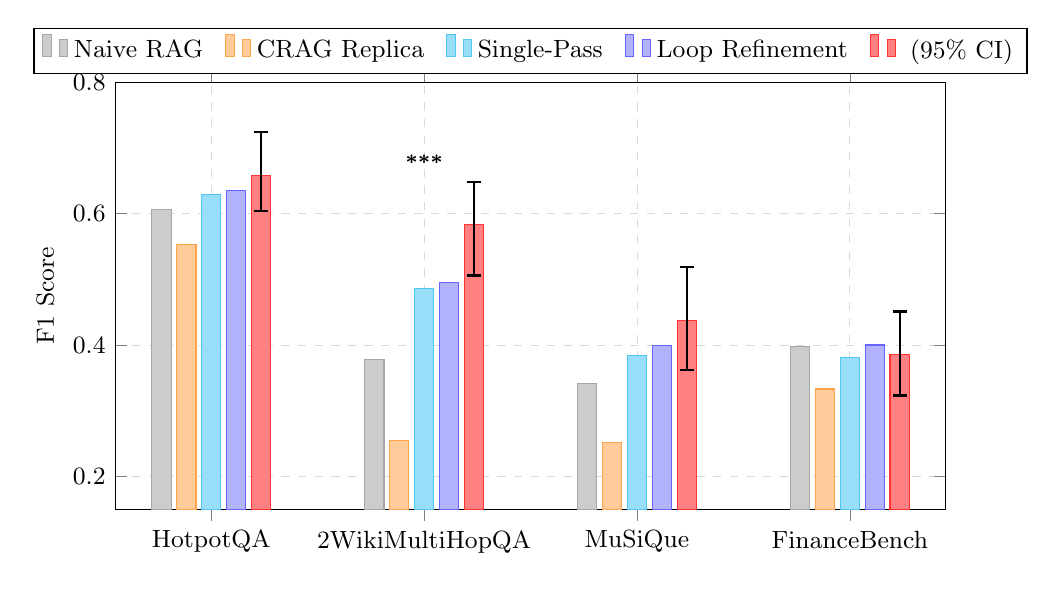
\begin{tikzpicture}
\begin{axis}[
    ybar,
    bar width=7pt,
    width=\textwidth,
    height=7cm,
    ylabel={F1 Score},
    symbolic x coords={HotpotQA, 2WikiMultiHopQA, MuSiQue, FinanceBench},
    xtick=data,
    ymin=0.15, ymax=0.80,
    legend style={
        at={(0.5,1.02)},
        anchor=south,
        legend columns=5,
        font=\small,
        /tikz/every even column/.append style={column sep=6pt}
    },
    ylabel style={font=\small},
    xticklabel style={font=\small},
    yticklabel style={font=\small},
    enlarge x limits=0.15,
    grid=major,
    grid style={dashed, gray!30},
    major grid style={line width=0.3pt},
]

% Naive RAG
\addplot[fill=gray!40, draw=gray!70] coordinates {
    (HotpotQA, 0.606)
    (2WikiMultiHopQA, 0.378)
    (MuSiQue, 0.342)
    (FinanceBench, 0.398)
};

% CRAG Replica
\addplot[fill=orange!40, draw=orange!70] coordinates {
    (HotpotQA, 0.553)
    (2WikiMultiHopQA, 0.255)
    (MuSiQue, 0.251)
    (FinanceBench, 0.333)
};

% Single-Pass
\addplot[fill=cyan!40, draw=cyan!70] coordinates {
    (HotpotQA, 0.630)
    (2WikiMultiHopQA, 0.486)
    (MuSiQue, 0.384)
    (FinanceBench, 0.381)
};

% Loop Refinement
\addplot[fill=blue!30, draw=blue!60] coordinates {
    (HotpotQA, 0.636)
    (2WikiMultiHopQA, 0.495)
    (MuSiQue, 0.399)
    (FinanceBench, 0.400)
};

% TARA (Agentic) with 95% bootstrap CI
% CI: Hot [.604,.725], 2Wiki [.506,.648], Mus [.362,.519], Fin [.323,.451]
% error minus = mean - lower, error plus = upper - mean
\addplot[
    fill=red!50, draw=red!80,
    error bars/.cd,
    y dir=both,
    y explicit,
    error bar style={black, thick},
    error mark options={rotate=90, mark size=2.5pt, thick},
] table [
    x=x, y=y,
    y error plus=ep,
    y error minus=em,
    col sep=comma,
] {
x,              y,     ep,    em
HotpotQA,       0.658, 0.067, 0.054
2WikiMultiHopQA,0.584, 0.064, 0.078
MuSiQue,        0.438, 0.081, 0.076
FinanceBench,   0.386, 0.065, 0.063
};

\legend{Naive RAG, CRAG Replica, Single-Pass, Loop Refinement, \ours{} (95\% CI)}

% Significance annotation
\node[font=\scriptsize\bfseries, anchor=south, yshift=1pt]
    at (axis cs:2WikiMultiHopQA, 0.648) {***};

\end{axis}
\end{tikzpicture}
\caption{F1 comparison across four datasets (Gemini Flash Lite, $n = 200$). \ours{} achieves the highest F1 on three of four datasets, with statistically significant improvement on 2WikiMultiHopQA ($p < 0.001$). Error bars on \ours{} indicate 95\% bootstrap confidence intervals (10,000 resamples; Table~\ref{tab:rq1_significance}). On FinanceBench, all iterative methods perform comparably (retrieval space saturation).}
\label{fig:rq1_f1}
\end{figure*}


\begin{table*}[t]
\centering
\caption{Main results (RQ1, Gemini Flash Lite). Best result per dataset in \textbf{bold}. $n = 200$ per dataset (FinanceBench: $n = 150$, full dataset). LLM-as-Judge uses gpt-4.1-nano as an independent evaluator.}
\label{tab:rq1_main}
\resizebox{\textwidth}{!}{%
\begin{tabular}{l ccc ccc ccc ccc}
\toprule
& \multicolumn{3}{c}{\textbf{HotpotQA}} & \multicolumn{3}{c}{\textbf{2WikiMultiHopQA}} & \multicolumn{3}{c}{\textbf{MuSiQue}} & \multicolumn{3}{c}{\textbf{FinanceBench}} \\
\cmidrule(lr){2-4} \cmidrule(lr){5-7} \cmidrule(lr){8-10} \cmidrule(lr){11-13}
\textbf{Pipeline} & EM & F1 & Judge & EM & F1 & Judge & EM & F1 & Judge & EM & F1 & Judge \\
\midrule
Naive RAG        & .445 & .606 & .700 & .275 & .378 & .400 & .235 & .342 & .335 & .167 & .398 & \textbf{.580} \\
CRAG Replica     & .400 & .553 & .645 & .130 & .255 & .320 & .175 & .251 & .225 & .107 & .333 & .487 \\
Single-Pass      & .470 & .630 & .720 & .375 & .486 & .495 & .280 & .384 & .360 & .160 & .381 & .507 \\
Loop Refinement  & .480 & .636 & .730 & .380 & .495 & .505 & .300 & .399 & .380 & \textbf{.180} & \textbf{.400} & .533 \\
\textbf{\ours{}} & \textbf{.505} & \textbf{.658} & \textbf{.765} & \textbf{.470} & \textbf{.584} & \textbf{.645} & \textbf{.330} & \textbf{.438} & \textbf{.405} & .153 & .386 & .527 \\
\midrule
\multicolumn{1}{r}{\textit{$\Delta$ vs.\ Loop}} & $+.025$ & $+.022$ & $+.035$ & $+.090$ & $+.089$ & $+.140$ & $+.030$ & $+.039$ & $+.025$ & $-.027$ & $-.014$ & $-.006$ \\
\bottomrule
\end{tabular}
}% end resizebox
\end{table*}

\paragraph{Complex multi-hop questions}
\ours{} achieves the best performance on both complex multi-hop datasets: 2WikiMultiHopQA (F1 0.584, $+0.089$ over Loop Refinement) and MuSiQue (F1 0.438, $+0.039$ over Loop).
These improvements are consistent across all three metrics (EM, F1, Judge), indicating genuine quality gains rather than metric-specific artifacts.
The LLM-as-Judge scores show the largest gaps on 2WikiMultiHopQA ($+0.140$), where the judge identifies correct multi-hop reasoning even when token overlap is moderate.
As we show in \S\ref{subsubsec:significance}, the 2WikiMultiHopQA improvement is statistically significant ($p < 0.001$) across all baseline comparisons.

\paragraph{Simple 2-hop questions}
On HotpotQA, \ours{} leads across all metrics (F1 0.658, EM 0.505, Judge 0.765), but the margin over Loop Refinement is small (F1 $+0.022$).
This suggests that 2-hop questions---where the required evidence can typically be retrieved in one or two search passes---do not fully exercise the agent's adaptive refinement capabilities.
The overhead of multi-step ReAct reasoning provides limited benefit when a single well-preprocessed retrieval pass is already sufficient.

\paragraph{Enterprise documents}
On FinanceBench, Loop Refinement marginally outperforms \ours{} in F1 (0.400 vs.\ 0.386, $\Delta = -0.014$) and EM (0.180 vs.\ 0.153).
Notably, Naive RAG achieves the highest Judge score (0.580), outperforming all iterative methods.
This pattern---where iterative refinement does \emph{not} improve and may slightly degrade answer quality---suggests a boundary condition for our approach.
We analyze this effect in detail in \S\ref{subsec:boundary}, attributing it to retrieval space saturation in FinanceBench's small corpus (211 passages).

\paragraph{CRAG Replica underperformance}
The CRAG Replica consistently ranks lowest, which is expected: our implementation replaces CRAG's web search fallback with internal re-retrieval (to match our enterprise-constrained setting) and uses LLM-based evaluation instead of a fine-tuned T5-large evaluator.
These architectural constraints substantially disadvantage the CRAG approach.

\paragraph{Key finding}
The agentic advantage is \emph{complexity-dependent}: improvements grow with question complexity (number of reasoning hops and retrieval difficulty), while simple questions and small-corpus settings show no benefit.
This pattern is consistent with the hypothesis that autonomous tool selection provides value primarily when the retrieval task requires adaptive strategy.

% ---------------------------------------------------------------------------
\subsubsection{Statistical Significance}
\label{subsubsec:significance}
% ---------------------------------------------------------------------------

To rigorously assess the reliability of observed differences, we perform paired bootstrap significance testing~\cite{efron1993bootstrap} with 10,000 resamples and Bonferroni correction for multiple comparisons.
Table~\ref{tab:rq1_significance} reports 95\% confidence intervals for \ours{} and pairwise comparisons against each baseline.

\begin{table*}[t]
\centering
\caption{Statistical significance (F1, paired bootstrap test, 10,000 resamples, Bonferroni-corrected $\alpha = 0.0125$). Top row: \ours{} F1 with 95\% bootstrap confidence interval. Lower rows: F1 difference $\Delta$ vs.\ each baseline (from Table~\ref{tab:rq1_main}); $p$-values from paired bootstrap. Significance: $^{***}p < 0.001$.}
\label{tab:rq1_significance}
\resizebox{\textwidth}{!}{%
\begin{tabular}{l cccc}
\toprule
& \textbf{HotpotQA} & \textbf{2WikiMultiHopQA} & \textbf{MuSiQue} & \textbf{FinanceBench} \\
\midrule
\ours{} F1 [95\% CI] & .658\;[.604,\;.725] & .584\;[.506,\;.648] & .438\;[.362,\;.519] & .386\;[.323,\;.451] \\
\midrule
$\Delta$ vs.\ Loop       & $+.022$           & $+.089^{***}$      & $+.039$           & $-.014$           \\
$\Delta$ vs.\ CRAG       & $+.105^{***}$     & $+.329^{***}$      & $+.187^{***}$     & $+.053$           \\
$\Delta$ vs.\ Single     & $+.028$           & $+.098^{***}$      & $+.054$           & $+.005$           \\
$\Delta$ vs.\ Naive      & $+.052$           & $+.206^{***}$      & $+.096^{***}$     & $-.012$           \\
\bottomrule
\end{tabular}
}% end resizebox
\end{table*}

\paragraph{2WikiMultiHopQA: strongest evidence}
\ours{} achieves statistically significant improvement over \emph{all four baselines} on 2WikiMultiHopQA ($p < 0.001$ in each case), with the largest effect against CRAG ($\Delta = +0.329$).
The 95\% confidence interval [$0.506, 0.648$] does not overlap with the confidence intervals of Loop [$0.433, 0.557$] or CRAG [$0.209, 0.305$], providing strong evidence that the improvement is not due to sampling variability.

\paragraph{MuSiQue: significant vs.\ weaker baselines}
Against CRAG ($+0.187$, $p < 0.001$) and Naive ($+0.096$, $p < 0.001$), the improvement is significant.
Against Loop ($+0.039$) and Single-Pass ($+0.054$), the positive trend does not reach significance, indicating that the refinement mechanisms converge for 3--4 hop questions that overlap in difficulty.

\paragraph{HotpotQA: comparable performance}
No pairwise comparison reaches significance except against CRAG ($+0.105$, $p < 0.001$), confirming that 2-hop questions do not discriminate between refinement approaches.

\paragraph{FinanceBench: no significant differences}
All pairwise comparisons are non-significant, with confidence intervals substantially overlapping.
The marginally negative delta against Loop ($-0.014$) is well within noise.
This statistical confirmation of the null result is consistent with the retrieval space saturation hypothesis discussed in \S\ref{subsec:boundary}.

% ---------------------------------------------------------------------------
\subsubsection{Cross-Model Validation}
\label{subsubsec:crossmodel}
% ---------------------------------------------------------------------------

To assess whether the observed patterns are model-dependent, we replicate the RQ1 experiment using gpt-5-mini\footnote{Model~ID: \texttt{gpt-5-mini}, with \texttt{reasoning\_effort=low}.}, a reasoning-oriented model from a different provider and architecture family.
Table~\ref{tab:rq1_crossmodel} presents the results.

\begin{table*}[t]
\centering
\caption{Cross-model validation (RQ1, gpt-5-mini). $n = 200$ per dataset (FinanceBench: $n = 150$). LLM-as-Judge: gpt-4.1-nano (same independent judge as Gemini experiments). Best per dataset in \textbf{bold}.}
\label{tab:rq1_crossmodel}
\resizebox{\textwidth}{!}{%
\begin{tabular}{l ccc ccc ccc ccc}
\toprule
& \multicolumn{3}{c}{\textbf{HotpotQA}} & \multicolumn{3}{c}{\textbf{2WikiMultiHopQA}} & \multicolumn{3}{c}{\textbf{MuSiQue}} & \multicolumn{3}{c}{\textbf{FinanceBench}} \\
\cmidrule(lr){2-4} \cmidrule(lr){5-7} \cmidrule(lr){8-10} \cmidrule(lr){11-13}
\textbf{Pipeline} & EM & F1 & Judge & EM & F1 & Judge & EM & F1 & Judge & EM & F1 & Judge \\
\midrule
Naive RAG        & .485 & .657 & .755 & .335 & .400 & .405 & .310 & .441 & .425 & .140 & .321 & \textbf{.540} \\
CRAG Replica     & \textbf{.535} & \textbf{.698} & .780 & \textbf{.550} & \textbf{.637} & \textbf{.655} & .370 & .491 & .460 & \textbf{.147} & \textbf{.343} & .520 \\
Single-Pass      & .505 & .678 & .735 & .390 & .465 & .485 & \textbf{.375} & .504 & .490 & .140 & .308 & .480 \\
Loop Refinement  & .510 & .689 & .750 & .425 & .510 & .540 & .370 & .505 & .485 & .160 & .328 & .507 \\
\textbf{\ours{}} & .510 & .697 & \textbf{.790} & .485 & .551 & .560 & \textbf{.375} & \textbf{.516} & \textbf{.505} & .133 & .317 & .513 \\
\midrule
\multicolumn{1}{r}{\textit{$\Delta$ vs.\ CRAG}} & $-.025$ & $-.001$ & $+.010$ & $-.065$ & $-.086$ & $-.095$ & $+.005$ & $+.025$ & $+.045$ & $-.014$ & $-.026$ & $-.007$ \\
\bottomrule
\end{tabular}
}% end resizebox
\end{table*}

\paragraph{Model--pipeline interaction effect}
The cross-model experiment reveals a striking reversal: with gpt-5-mini, CRAG Replica outperforms \ours{} on 2WikiMultiHopQA (F1 0.637 vs.\ 0.551, $p = 0.004$) and FinanceBench (F1 0.343 vs.\ 0.317, $p = 0.042$).
This contrasts sharply with the Gemini results, where \ours{} leads on both datasets.
The reversal is driven by what we term \emph{Reasoning Model Refusal Asymmetry}: the reasoning capabilities of gpt-5-mini lead it to apply higher evidentiary standards within the ReAct framework, resulting in a 30\% answer refusal rate on 2WikiMultiHopQA (compared to 18\% for CRAG).
CRAG's rigid judge--correct--generate pipeline precludes refusal, ensuring an answer is always produced.
We analyze this phenomenon in detail in \S\ref{subsec:model_interaction}.

\paragraph{Consistent findings}
Despite the model--pipeline interaction, several patterns remain consistent across both models:
(1)~\ours{} leads on MuSiQue (F1 0.516, Judge 0.505), the hardest multi-hop dataset;
(2)~Naive RAG achieves the highest Judge score on FinanceBench with both models (0.580 for Gemini, 0.540 for gpt-5-mini);
(3)~HotpotQA shows compressed performance ranges with both models.
The LLM-as-Judge also resolves an apparent tie on HotpotQA: \ours{} achieves 0.790 vs.\ CRAG's 0.780, suggesting subtle quality advantages that F1 cannot capture.

% ---------------------------------------------------------------------------
\subsubsection{Latency Analysis}
\label{subsubsec:latency}
% ---------------------------------------------------------------------------

Table~\ref{tab:latency} reports average per-question latency for the Gemini configuration.

\begin{table}[t]
\centering
\caption{Average latency per question (seconds, Gemini Flash Lite, $\tau = 40$). Latency is dominated by LLM API calls; the agent averages 5--6 tool invocations per question.}
\label{tab:latency}
\begin{tabular}{lcccc}
\toprule
\textbf{Pipeline} & \textbf{HotpotQA} & \textbf{2Wiki} & \textbf{MuSiQue} & \textbf{Finance} \\
\midrule
Naive RAG       & 0.5 & 0.3 & 0.3 & 0.3 \\
CRAG Replica    & 0.4 & 0.1 & 0.1 & 0.1 \\
Single-Pass     & 4.2 & 3.0 & 3.5 & 4.9 \\
Loop Refinement & 3.1 & 1.7 & 3.6 & 2.7 \\
\textbf{\ours{}} & 14.9 & 13.6 & 15.2 & 16.8 \\
\bottomrule
\end{tabular}
\end{table}

\ours{} requires 14--17 seconds per question, approximately 4--5$\times$ slower than Loop Refinement and 30--50$\times$ slower than Naive RAG.
This overhead stems from the ReAct reasoning loop: each iteration involves LLM inference for thought generation, tool selection, and observation processing.
With an average of 5.4--6.2 tool calls per question (see \S\ref{subsec:rq2}), the agent performs substantially more LLM calls than the fixed-loop approach.
With gpt-5-mini, latency increases further to 45.7s per question on 2WikiMultiHopQA due to the model's reasoning overhead. CRAG requires 147.8s per question with gpt-5-mini, as its multi-stage pipeline involves 45.2 LLM calls per question.
We discuss the latency--quality trade-off and practical implications in \S\ref{sec:discussion}.

% ---------------------------------------------------------------------------
\subsection{RQ2: Tool Usage and Trajectory Analysis}
\label{subsec:rq2}
% ---------------------------------------------------------------------------

\textbf{How does the ReAct agent use its tools, and what behavioral patterns emerge?}

% ---------------------------------------------------------------------------
\subsubsection{Tool Frequency}
\label{subsubsec:tool_freq}
% ---------------------------------------------------------------------------

Table~\ref{tab:tool_usage} and Figure~\ref{fig:tool_usage} report the average number of tool calls per question across all four datasets.

% Figure: Tool Usage Heatmap (RQ2)
\begin{figure}[t]
\centering
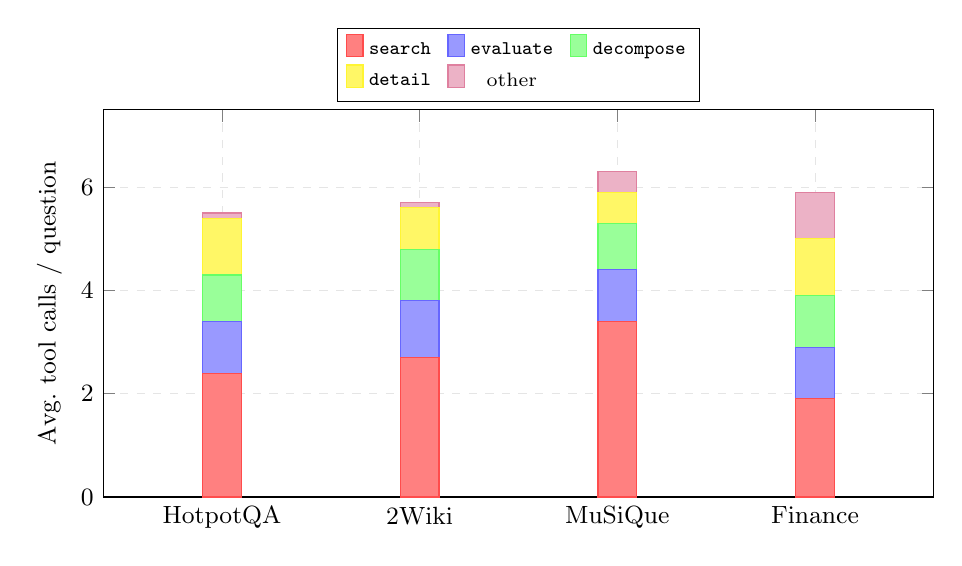
\begin{tikzpicture}
\begin{axis}[
    ybar stacked,
    bar width=14pt,
    width=\columnwidth,
    height=6.5cm,
    ylabel={Avg.\ tool calls / question},
    symbolic x coords={HotpotQA, 2Wiki, MuSiQue, Finance},
    xtick=data,
    xticklabel style={font=\small},
    ylabel style={font=\small},
    yticklabel style={font=\small},
    ymin=0, ymax=7.5,
    legend style={
        at={(0.5,1.02)},
        anchor=south,
        legend columns=3,
        font=\scriptsize,
        /tikz/every even column/.append style={column sep=4pt}
    },
    enlarge x limits=0.2,
    grid=major,
    grid style={dashed, gray!20},
    major grid style={line width=0.2pt},
]

% search_passages
\addplot[fill=red!50, draw=red!70] coordinates {
    (HotpotQA, 2.4)
    (2Wiki, 2.7)
    (MuSiQue, 3.4)
    (Finance, 1.9)
};

% evaluate_passages
\addplot[fill=blue!40, draw=blue!60] coordinates {
    (HotpotQA, 1.0)
    (2Wiki, 1.1)
    (MuSiQue, 1.0)
    (Finance, 1.0)
};

% decompose_query
\addplot[fill=green!40, draw=green!60] coordinates {
    (HotpotQA, 0.9)
    (2Wiki, 1.0)
    (MuSiQue, 0.9)
    (Finance, 1.0)
};

% get_passage_detail
\addplot[fill=yellow!60, draw=yellow!80] coordinates {
    (HotpotQA, 1.1)
    (2Wiki, 0.8)
    (MuSiQue, 0.6)
    (Finance, 1.1)
};

% list_sections + calculate + terminology (grouped as "other")
\addplot[fill=purple!30, draw=purple!50] coordinates {
    (HotpotQA, 0.1)
    (2Wiki, 0.1)
    (MuSiQue, 0.4)
    (Finance, 0.9)
};

\legend{\texttt{search}, \texttt{evaluate}, \texttt{decompose}, \texttt{detail}, other}

\end{axis}
\end{tikzpicture}
\caption{Tool call distribution per question (RQ2, $n = 200$). Search dominates across all datasets, with MuSiQue requiring the most tool calls (6.2/q) due to its 3--4 hop complexity. FinanceBench shows the most diverse tool usage, including domain-specific \texttt{calculate} and \texttt{list\_sections} (grouped as ``other'').}
\label{fig:tool_usage}
\end{figure}


\begin{table}[t]
\centering
\caption{Average tool calls per question ($n = 200$ per dataset). The agent prioritizes search and decomposition, with evaluation called at least once per question via mandatory fallback.}
\label{tab:tool_usage}
\begin{tabular}{lcccc}
\toprule
\textbf{Tool} & \textbf{HotpotQA} & \textbf{2Wiki} & \textbf{MuSiQue} & \textbf{Finance} \\
\midrule
\texttt{search\_passages}          & 2.4 & 2.7 & 3.4 & 1.9 \\
\texttt{evaluate\_passages}        & 1.0 & 1.1 & 1.0 & 1.0 \\
\texttt{decompose\_query}          & 0.9 & 1.0 & 0.9 & 1.0 \\
\texttt{get\_passage\_detail}      & 1.1 & 0.8 & 0.6 & 1.1 \\
\texttt{list\_document\_sections}  & 0.1 & 0.1 & 0.4 & 0.5 \\
\texttt{calculate}                 & --  & --  & --  & 0.4 \\
\texttt{get\_terminology}          & $<$0.1 & 0.0 & $<$0.1 & $<$0.1 \\
\midrule
\textbf{Total tools/question} & \textbf{5.4} & \textbf{5.7} & \textbf{6.2} & \textbf{5.8} \\
\bottomrule
\end{tabular}
\end{table}

\paragraph{Search dominance}
The agent calls \texttt{search\_passages} 1.9--3.4 times per question, making it the most frequently used tool.
MuSiQue exhibits the highest search frequency (3.4), consistent with its 3--4 hop structure requiring multiple independent evidence retrieval passes.
Conversely, FinanceBench requires the fewest searches (1.9), reflecting its small corpus where initial retrieval often suffices.

\paragraph{Progressive information disclosure}
\texttt{get\_passage\_detail} is called 0.6--1.1 times per question, indicating that the agent actively employs a two-stage retrieval strategy: first scanning search previews (200-character summaries), then retrieving full text for promising passages.
This progressive disclosure reduces context window consumption while maintaining retrieval precision.

\paragraph{Structure-aware navigation}
\texttt{list\_document\_sections} is rarely used on Wikipedia-based datasets ($\leq 0.1$ per question) but more frequently on MuSiQue (0.4 per question) and FinanceBench (0.5 per question), where complex document structures benefit from hierarchical navigation.
In contrast, \texttt{get\_terminology} is virtually unused across all datasets ($< 0.1$ calls per question), indicating that the vocabulary gap between questions and corpus language is not a significant bottleneck for these benchmarks.

\paragraph{Domain-adaptive tool selection}
On FinanceBench, the agent invokes \texttt{calculate} (0.4 calls per question) for numerical computations such as margin calculations and year-over-year comparisons.
This tool is completely unused on Wikipedia-based datasets, demonstrating the agent's ability to adapt its tool repertoire to the domain without explicit configuration.

% ---------------------------------------------------------------------------
\subsubsection{Trajectory Patterns}
\label{subsubsec:trajectories}
% ---------------------------------------------------------------------------

Analysis of ReAct trajectories reveals three dominant behavioral patterns:

\begin{enumerate}
    \item \textbf{Decompose--Search--Evaluate} (most common): The agent decomposes the question into sub-questions, searches each independently, and evaluates the combined passage set. This is the canonical multi-hop retrieval strategy.

    \item \textbf{Search--Evaluate} (simple cases): For questions identified as single-hop, the agent skips decomposition and directly searches with the preprocessed query before evaluating.

    \item \textbf{Decompose--Search--Evaluate--Refine} (iterative refinement): When the initial evaluation score falls below the quality threshold, the agent uses evaluation feedback to refine the query, performs an additional search, and re-evaluates.
\end{enumerate}

Notably, the agent \emph{converges on} these structured protocols through ReAct reasoning, despite having access to a broader set of tools and no hard-coded execution sequence.
The protocol is suggested in the agent's signature docstring but not enforced---the agent could deviate but consistently converges on these patterns across all 800+ questions evaluated.

% ---------------------------------------------------------------------------
\subsection{RQ5: DSPy Optimization Effect}
\label{subsec:rq5}
% ---------------------------------------------------------------------------

\textbf{Does DSPy's declarative pipeline and automatic optimization improve answer quality compared to manual prompt engineering?}

Table~\ref{tab:rq5} compares four prompt engineering approaches.
The test set sizes ($N$) differ from RQ1 because 50 examples per dataset are reserved for DSPy optimization training and 20 for validation.

\begin{table*}[t]
\centering
\caption{DSPy optimization results (RQ5, Gemini Flash Lite). ``Manual'' uses hand-crafted JSON templates; ``Unopt'' uses DSPy typed Signatures without optimization; Bootstrap and MIPROv2 add automatic few-shot/instruction optimization. Best per dataset in \textbf{bold}. $N$: test set size after train/validation split.}
\label{tab:rq5}
\resizebox{\textwidth}{!}{%
\begin{tabular}{l cc cc cc cc c}
\toprule
& \multicolumn{2}{c}{\textbf{HotpotQA}} & \multicolumn{2}{c}{\textbf{2WikiMultiHopQA}} & \multicolumn{2}{c}{\textbf{MuSiQue}} & \multicolumn{2}{c}{\textbf{FinanceBench}} & \\
\cmidrule(lr){2-3} \cmidrule(lr){4-5} \cmidrule(lr){6-7} \cmidrule(lr){8-9}
\textbf{Variant} & EM & F1 & EM & F1 & EM & F1 & EM & F1 & $N$ \\
\midrule
Manual Prompt       & .408 & .587 & .308 & .476 & .338 & .466 & .013 & .255 & -- \\
DSPy Unopt          & .508 & .658 & .485 & .602 & .300 & .396 & .188 & .419 & -- \\
DSPy + Bootstrap    & \textbf{.508} & \textbf{.664} & \textbf{.554} & \textbf{.646} & \textbf{.469} & \textbf{.544} & \textbf{.200} & \textbf{.431} & 130/80 \\
DSPy + MIPROv2      & .500 & .655 & .400 & .528 & .423 & .503 & .175 & .409 & 130/80 \\
\midrule
\multicolumn{1}{r}{\textit{$\Delta$ Manual$\to$Unopt}} & $+.100$ & $+.071$ & $+.177$ & $+.126$ & $-.038$ & $-.070$ & $+.175$ & $+.164$ & \\
\multicolumn{1}{r}{\textit{$\Delta$ Manual$\to$Best}} & $+.100$ & $+.077$ & $+.246$ & $+.170$ & $+.131$ & $+.078$ & $+.187$ & $+.176$ & \\
\bottomrule
\end{tabular}
}% end resizebox
\end{table*}

\paragraph{Structural benefit: Manual $\to$ DSPy Unopt}
Replacing hand-crafted JSON prompt templates with DSPy typed Signatures yields substantial improvements \emph{without any optimization} on three datasets: F1 increases of $+0.071$ (HotpotQA), $+0.126$ (2WikiMultiHopQA), and $+0.164$ (FinanceBench).
The FinanceBench improvement is particularly notable: from F1 0.255 to 0.419, with EM increasing from 0.013 to 0.188.
MuSiQue is the exception, where Unopt substantially underperforms Manual ($-0.070$ F1), suggesting that DSPy's structured output constraints can conflict with question patterns that benefit from free-form generation.
This dataset-dependent variance highlights that the structural benefit is not universal but depends on alignment between typed Signature constraints and task characteristics.

\paragraph{Optimization benefit: Unopt $\to$ Bootstrap/MIPROv2}
Automatic optimization provides additional gains, but the effect is \emph{dataset-dependent}:

\begin{itemize}
    \item \textbf{BootstrapFewShot} is the most consistently effective optimizer, achieving the best F1 on all four datasets: HotpotQA (0.664, $+0.006$ over Unopt), 2WikiMultiHopQA (0.646, $+0.044$), MuSiQue (0.544, $+0.148$), and FinanceBench (0.431, $+0.012$). The large MuSiQue gain ($+0.148$) demonstrates that few-shot examples from successful execution traces can recover performance lost by the Unopt variant's rigid structure.

    \item \textbf{MIPROv2} provides strong gains on MuSiQue (0.503, $+0.107$ over Unopt) but underperforms Bootstrap on the remaining datasets. The jointly optimized instructions appear most beneficial for complex reasoning chains.

    \item \textbf{Optimization rescues structural mismatch}: On MuSiQue, where Unopt underperforms Manual, both optimizers substantially surpass Manual (Bootstrap $+0.078$, MIPROv2 $+0.037$ F1), demonstrating that automatic optimization can compensate for suboptimal Signature--task alignment.
\end{itemize}

\paragraph{Key finding}
DSPy provides a two-level contribution: (1) the \emph{structural benefit} of typed Signatures yields F1 improvements of $+0.071$--$0.164$ on three of four datasets, and (2) automatic optimization provides additional gains, with BootstrapFewShot achieving the best F1 on all four datasets.
Critically, optimization can rescue structural mismatch: on MuSiQue, where Unopt underperforms Manual, Bootstrap still achieves the overall best F1 ($+0.078$ over Manual).
The total improvement from Manual to best DSPy variant ranges from $+0.077$ to $+0.176$ F1, supporting the practical value of declarative LM programming for RAG systems.
